\documentclass[twoside]{book}

% Packages required by doxygen
\usepackage{calc}
\usepackage{doxygen}
\usepackage{graphicx}
\usepackage[utf8]{inputenc}
\usepackage{makeidx}
\usepackage{multicol}
\usepackage{multirow}
\usepackage{textcomp}
\usepackage[table]{xcolor}

% Font selection
\usepackage[T1]{fontenc}
\usepackage{mathptmx}
\usepackage[scaled=.90]{helvet}
\usepackage{courier}
\usepackage{amssymb}
\usepackage{sectsty}
\renewcommand{\familydefault}{\sfdefault}
\allsectionsfont{%
  \fontseries{bc}\selectfont%
  \color{darkgray}%
}
\renewcommand{\DoxyLabelFont}{%
  \fontseries{bc}\selectfont%
  \color{darkgray}%
}

% Page & text layout
\usepackage{geometry}
\geometry{%
  a4paper,%
  top=2.5cm,%
  bottom=2.5cm,%
  left=2.5cm,%
  right=2.5cm%
}
\tolerance=750
\hfuzz=15pt
\hbadness=750
\setlength{\emergencystretch}{15pt}
\setlength{\parindent}{0cm}
\setlength{\parskip}{0.2cm}
\makeatletter
\renewcommand{\paragraph}{%
  \@startsection{paragraph}{4}{0ex}{-1.0ex}{1.0ex}{%
    \normalfont\normalsize\bfseries\SS@parafont%
  }%
}
\renewcommand{\subparagraph}{%
  \@startsection{subparagraph}{5}{0ex}{-1.0ex}{1.0ex}{%
    \normalfont\normalsize\bfseries\SS@subparafont%
  }%
}
\makeatother

% Headers & footers
\usepackage{fancyhdr}
\pagestyle{fancyplain}
\fancyhead[LE]{\fancyplain{}{\bfseries\thepage}}
\fancyhead[CE]{\fancyplain{}{}}
\fancyhead[RE]{\fancyplain{}{\bfseries\leftmark}}
\fancyhead[LO]{\fancyplain{}{\bfseries\rightmark}}
\fancyhead[CO]{\fancyplain{}{}}
\fancyhead[RO]{\fancyplain{}{\bfseries\thepage}}
\fancyfoot[LE]{\fancyplain{}{}}
\fancyfoot[CE]{\fancyplain{}{}}
\fancyfoot[RE]{\fancyplain{}{\bfseries\scriptsize Generated on Mon Mar 23 2015 00\-:33\-:08 for My Project by Doxygen }}
\fancyfoot[LO]{\fancyplain{}{\bfseries\scriptsize Generated on Mon Mar 23 2015 00\-:33\-:08 for My Project by Doxygen }}
\fancyfoot[CO]{\fancyplain{}{}}
\fancyfoot[RO]{\fancyplain{}{}}
\renewcommand{\footrulewidth}{0.4pt}
\renewcommand{\chaptermark}[1]{%
  \markboth{#1}{}%
}
\renewcommand{\sectionmark}[1]{%
  \markright{\thesection\ #1}%
}

% Indices & bibliography
\usepackage{natbib}
\usepackage[titles]{tocloft}
\setcounter{tocdepth}{3}
\setcounter{secnumdepth}{5}
\makeindex

% Hyperlinks (required, but should be loaded last)
\usepackage{ifpdf}
\ifpdf
  \usepackage[pdftex,pagebackref=true]{hyperref}
\else
  \usepackage[ps2pdf,pagebackref=true]{hyperref}
\fi
\hypersetup{%
  colorlinks=true,%
  linkcolor=blue,%
  citecolor=blue,%
  unicode%
}

% Custom commands
\newcommand{\clearemptydoublepage}{%
  \newpage{\pagestyle{empty}\cleardoublepage}%
}


%===== C O N T E N T S =====

\begin{document}

% Titlepage & ToC
\hypersetup{pageanchor=false}
\pagenumbering{roman}
\begin{titlepage}
\vspace*{7cm}
\begin{center}%
{\Large My Project }\\
\vspace*{1cm}
{\large Generated by Doxygen 1.8.5}\\
\vspace*{0.5cm}
{\small Mon Mar 23 2015 00:33:08}\\
\end{center}
\end{titlepage}
\clearemptydoublepage
\tableofcontents
\clearemptydoublepage
\pagenumbering{arabic}
\hypersetup{pageanchor=true}

%--- Begin generated contents ---
\chapter{project\-\_\-brickbreaker}
\label{md_README}
\hypertarget{md_README}{}
\input{md_README}
\chapter{Hierarchical Index}
\section{Class Hierarchy}
This inheritance list is sorted roughly, but not completely, alphabetically\-:\begin{DoxyCompactList}
\item \contentsline{section}{bloc}{\pageref{structbloc}}{}
\begin{DoxyCompactList}
\item \contentsline{section}{raquette}{\pageref{classraquette}}{}
\end{DoxyCompactList}
\item \contentsline{section}{cibles}{\pageref{structcibles}}{}
\item \contentsline{section}{circle}{\pageref{structcircle}}{}
\item Q\-Main\-Window\begin{DoxyCompactList}
\item \contentsline{section}{window}{\pageref{classwindow}}{}
\end{DoxyCompactList}
\item Q\-Widget\begin{DoxyCompactList}
\item \contentsline{section}{render\-\_\-area}{\pageref{classrender__area}}{}
\end{DoxyCompactList}
\item \contentsline{section}{vec2}{\pageref{structvec2}}{}
\end{DoxyCompactList}

\chapter{Class Index}
\section{Class List}
Here are the classes, structs, unions and interfaces with brief descriptions\-:\begin{DoxyCompactList}
\item\contentsline{section}{\hyperlink{structbloc}{bloc} \\*The bloc struct }{\pageref{structbloc}}{}
\item\contentsline{section}{\hyperlink{structcibles}{cibles} \\*The cibles struct }{\pageref{structcibles}}{}
\item\contentsline{section}{\hyperlink{structcircle}{circle} }{\pageref{structcircle}}{}
\item\contentsline{section}{\hyperlink{classraquette}{raquette} }{\pageref{classraquette}}{}
\item\contentsline{section}{\hyperlink{classrender__area}{render\-\_\-area} }{\pageref{classrender__area}}{}
\item\contentsline{section}{\hyperlink{structvec2}{vec2} }{\pageref{structvec2}}{}
\item\contentsline{section}{\hyperlink{classwindow}{window} }{\pageref{classwindow}}{}
\end{DoxyCompactList}

\chapter{Class Documentation}
\hypertarget{structbloc}{\section{bloc Struct Reference}
\label{structbloc}\index{bloc@{bloc}}
}


The bloc struct.  




{\ttfamily \#include $<$bloc.\-hpp$>$}

\subsection*{Public Member Functions}
\begin{DoxyCompactItemize}
\item 
\hyperlink{structbloc_a2a5a4e418a9decebe5b7f30df71af385}{bloc} (\hyperlink{structvec2}{vec2} origine, float Longeur, float Hauteur)
\begin{DoxyCompactList}\small\item\em bloc \end{DoxyCompactList}\item 
bool \hyperlink{structbloc_a51aa6ddde5ddfec73ab1ac6004a1e09c}{est\-Toucher} (\hyperlink{structcircle}{circle} const \&balle)
\begin{DoxyCompactList}\small\item\em est\-Toucher /$\ast$$\ast$ $\ast$ \end{DoxyCompactList}\item 
bool \hyperlink{structbloc_a731b8b1d5fe6c1cf9e0edcc5c5cccc1b}{operator==} (\hyperlink{structbloc}{bloc} const \&A)
\begin{DoxyCompactList}\small\item\em operator == \end{DoxyCompactList}\end{DoxyCompactItemize}
\subsection*{Public Attributes}
\begin{DoxyCompactItemize}
\item 
\hyperlink{structvec2}{vec2} \hyperlink{structbloc_a66f43d85d906eae25ff2bd055704ec76}{bas\-\_\-gauche}
\item 
float \hyperlink{structbloc_a952b25540dde128110d4c1046656cb5e}{L}
\item 
\hypertarget{structbloc_a59981ef09d24dcf015f480c3e4318eef}{float {\bfseries H}}\label{structbloc_a59981ef09d24dcf015f480c3e4318eef}

\end{DoxyCompactItemize}


\subsection{Detailed Description}
The bloc struct. 

\subsection{Constructor \& Destructor Documentation}
\hypertarget{structbloc_a2a5a4e418a9decebe5b7f30df71af385}{\index{bloc@{bloc}!bloc@{bloc}}
\index{bloc@{bloc}!bloc@{bloc}}
\subsubsection[{bloc}]{\setlength{\rightskip}{0pt plus 5cm}bloc\-::bloc (
\begin{DoxyParamCaption}
\item[{{\bf vec2}}]{origine, }
\item[{float}]{Longeur, }
\item[{float}]{Hauteur}
\end{DoxyParamCaption}
)}}\label{structbloc_a2a5a4e418a9decebe5b7f30df71af385}


bloc 


\begin{DoxyParams}{Parameters}
{\em origine} & \\
\hline
{\em Longeur} & \\
\hline
{\em Hauteur} & Constructeur d'un bloc \\
\hline
\end{DoxyParams}


\subsection{Member Function Documentation}
\hypertarget{structbloc_a51aa6ddde5ddfec73ab1ac6004a1e09c}{\index{bloc@{bloc}!est\-Toucher@{est\-Toucher}}
\index{est\-Toucher@{est\-Toucher}!bloc@{bloc}}
\subsubsection[{est\-Toucher}]{\setlength{\rightskip}{0pt plus 5cm}bool bloc\-::est\-Toucher (
\begin{DoxyParamCaption}
\item[{{\bf circle} const \&}]{balle}
\end{DoxyParamCaption}
)}}\label{structbloc_a51aa6ddde5ddfec73ab1ac6004a1e09c}


est\-Toucher /$\ast$$\ast$ $\ast$ 

\hyperlink{structbloc_a51aa6ddde5ddfec73ab1ac6004a1e09c}{bloc\-::est\-Toucher} /$\ast$$\ast$ $\ast$

/$\ast$$\ast$ $\ast$ 
\begin{DoxyParams}{Parameters}
{\em balle} & /$\ast$$\ast$ $\ast$ \\
\hline
\end{DoxyParams}
\begin{DoxyReturn}{Returns}
/$\ast$$\ast$
\end{DoxyReturn}
/$\ast$$\ast$ $\ast$ 
\begin{DoxyParams}{Parameters}
{\em balle} & /$\ast$$\ast$ $\ast$ \\
\hline
\end{DoxyParams}
\begin{DoxyReturn}{Returns}
permet de determiné si le bloc a été toucher par la balle /$\ast$$\ast$ 
\end{DoxyReturn}
\hypertarget{structbloc_a731b8b1d5fe6c1cf9e0edcc5c5cccc1b}{\index{bloc@{bloc}!operator==@{operator==}}
\index{operator==@{operator==}!bloc@{bloc}}
\subsubsection[{operator==}]{\setlength{\rightskip}{0pt plus 5cm}bool bloc\-::operator== (
\begin{DoxyParamCaption}
\item[{{\bf bloc} const \&}]{A}
\end{DoxyParamCaption}
)}}\label{structbloc_a731b8b1d5fe6c1cf9e0edcc5c5cccc1b}


operator == 


\begin{DoxyParams}{Parameters}
{\em A} & \\
\hline
\end{DoxyParams}
\begin{DoxyReturn}{Returns}

\end{DoxyReturn}


\subsection{Member Data Documentation}
\hypertarget{structbloc_a66f43d85d906eae25ff2bd055704ec76}{\index{bloc@{bloc}!bas\-\_\-gauche@{bas\-\_\-gauche}}
\index{bas\-\_\-gauche@{bas\-\_\-gauche}!bloc@{bloc}}
\subsubsection[{bas\-\_\-gauche}]{\setlength{\rightskip}{0pt plus 5cm}{\bf vec2} bloc\-::bas\-\_\-gauche}}\label{structbloc_a66f43d85d906eae25ff2bd055704ec76}
Origine du bloc (en bas à gauche) \hypertarget{structbloc_a952b25540dde128110d4c1046656cb5e}{\index{bloc@{bloc}!L@{L}}
\index{L@{L}!bloc@{bloc}}
\subsubsection[{L}]{\setlength{\rightskip}{0pt plus 5cm}float bloc\-::\-L}}\label{structbloc_a952b25540dde128110d4c1046656cb5e}
L=largeur H=hauteur 

The documentation for this struct was generated from the following files\-:\begin{DoxyCompactItemize}
\item 
bloc.\-hpp\item 
bloc.\-cpp\end{DoxyCompactItemize}

\hypertarget{structcibles}{\section{cibles Struct Reference}
\label{structcibles}\index{cibles@{cibles}}
}


The cibles struct.  




{\ttfamily \#include $<$cibles.\-hpp$>$}

\subsection*{Public Member Functions}
\begin{DoxyCompactItemize}
\item 
\hypertarget{structcibles_aff3b848ce81ad0ce76482844a6ad3ac1}{\hyperlink{structcibles_aff3b848ce81ad0ce76482844a6ad3ac1}{cibles} ()}\label{structcibles_aff3b848ce81ad0ce76482844a6ad3ac1}

\begin{DoxyCompactList}\small\item\em cibles \end{DoxyCompactList}\item 
\hyperlink{structcibles_a638f2d963ebfaf52e64608ed629311bc}{cibles} (int N, int nombre\-Lignes, Q\-Widget zone\-\_\-de\-\_\-jeu)
\begin{DoxyCompactList}\small\item\em cibles \end{DoxyCompactList}\item 
void \hyperlink{structcibles_a361b3e39738fcc849de170d392a65b6c}{gestion\-Collision} (\hyperlink{structcircle}{circle} const \&balle)
\begin{DoxyCompactList}\small\item\em gestion\-Collision \end{DoxyCompactList}\end{DoxyCompactItemize}
\subsection*{Public Attributes}
\begin{DoxyCompactItemize}
\item 
\hypertarget{structcibles_a5882b203001202b7cf98bb57f54638d5}{int \hyperlink{structcibles_a5882b203001202b7cf98bb57f54638d5}{nombre\-Cibles}}\label{structcibles_a5882b203001202b7cf98bb57f54638d5}

\begin{DoxyCompactList}\small\item\em nombre\-Cibles \end{DoxyCompactList}\item 
\hypertarget{structcibles_ac5061cda0bf0b1709c149b55f79f8eec}{std\-::list$<$ \hyperlink{structbloc}{bloc} $>$ {\bfseries briques}}\label{structcibles_ac5061cda0bf0b1709c149b55f79f8eec}

\end{DoxyCompactItemize}


\subsection{Detailed Description}
The cibles struct. 

\subsection{Constructor \& Destructor Documentation}
\hypertarget{structcibles_a638f2d963ebfaf52e64608ed629311bc}{\index{cibles@{cibles}!cibles@{cibles}}
\index{cibles@{cibles}!cibles@{cibles}}
\subsubsection[{cibles}]{\setlength{\rightskip}{0pt plus 5cm}cibles\-::cibles (
\begin{DoxyParamCaption}
\item[{int}]{N, }
\item[{int}]{nombre\-Lignes, }
\item[{Q\-Widget}]{zone\-\_\-de\-\_\-jeu}
\end{DoxyParamCaption}
)}}\label{structcibles_a638f2d963ebfaf52e64608ed629311bc}


cibles 


\begin{DoxyParams}{Parameters}
{\em N} & \\
\hline
{\em nombre\-Lignes} & \\
\hline
{\em zone\-\_\-de\-\_\-jeu} & Constructeur permettant de genérer une matrice de N element qui remplis toute la partie haute de l'élément \\
\hline
\end{DoxyParams}


\subsection{Member Function Documentation}
\hypertarget{structcibles_a361b3e39738fcc849de170d392a65b6c}{\index{cibles@{cibles}!gestion\-Collision@{gestion\-Collision}}
\index{gestion\-Collision@{gestion\-Collision}!cibles@{cibles}}
\subsubsection[{gestion\-Collision}]{\setlength{\rightskip}{0pt plus 5cm}void cibles\-::gestion\-Collision (
\begin{DoxyParamCaption}
\item[{{\bf circle} const \&}]{balle}
\end{DoxyParamCaption}
)}}\label{structcibles_a361b3e39738fcc849de170d392a65b6c}


gestion\-Collision 


\begin{DoxyParams}{Parameters}
{\em balle} & \\
\hline
\end{DoxyParams}


The documentation for this struct was generated from the following files\-:\begin{DoxyCompactItemize}
\item 
cibles.\-hpp\item 
cibles.\-cpp\end{DoxyCompactItemize}

\hypertarget{structcircle}{\section{circle Struct Reference}
\label{structcircle}\index{circle@{circle}}
}


{\ttfamily \#include $<$circle.\-hpp$>$}

\subsection*{Public Member Functions}
\begin{DoxyCompactItemize}
\item 
\hyperlink{structcircle_a4e0786fc75051f3bbe5de2e08ef9712d}{circle} ()
\item 
\hyperlink{structcircle_a13bd963deb70b1ef5e5747c3478ef551}{circle} (\hyperlink{structvec2}{vec2} const \&center\-\_\-param, float radius\-\_\-center)
\item 
\hypertarget{structcircle_a1ce5660cf29852bee97341cfefa03655}{\hyperlink{structvec2}{vec2} {\bfseries get\-Coord} ()}\label{structcircle_a1ce5660cf29852bee97341cfefa03655}

\end{DoxyCompactItemize}
\subsection*{Public Attributes}
\begin{DoxyCompactItemize}
\item 
\hyperlink{structvec2}{vec2} \hyperlink{structcircle_ae816534fba5132b6db750022a50cc35e}{center}
\item 
float \hyperlink{structcircle_a4724daa580ad7e0516ba108cb2a41364}{radius}
\end{DoxyCompactItemize}


\subsection{Detailed Description}
A structure containing parameter of a geometric circle 

\subsection{Constructor \& Destructor Documentation}
\hypertarget{structcircle_a4e0786fc75051f3bbe5de2e08ef9712d}{\index{circle@{circle}!circle@{circle}}
\index{circle@{circle}!circle@{circle}}
\subsubsection[{circle}]{\setlength{\rightskip}{0pt plus 5cm}circle\-::circle (
\begin{DoxyParamCaption}
{}
\end{DoxyParamCaption}
)}}\label{structcircle_a4e0786fc75051f3bbe5de2e08ef9712d}
Constructor circle (0,0) \hypertarget{structcircle_a13bd963deb70b1ef5e5747c3478ef551}{\index{circle@{circle}!circle@{circle}}
\index{circle@{circle}!circle@{circle}}
\subsubsection[{circle}]{\setlength{\rightskip}{0pt plus 5cm}circle\-::circle (
\begin{DoxyParamCaption}
\item[{{\bf vec2} const \&}]{center\-\_\-param, }
\item[{float}]{radius\-\_\-center}
\end{DoxyParamCaption}
)}}\label{structcircle_a13bd963deb70b1ef5e5747c3478ef551}
Constructor circle (\{x,y\},R) 

\subsection{Member Data Documentation}
\hypertarget{structcircle_ae816534fba5132b6db750022a50cc35e}{\index{circle@{circle}!center@{center}}
\index{center@{center}!circle@{circle}}
\subsubsection[{center}]{\setlength{\rightskip}{0pt plus 5cm}{\bf vec2} circle\-::center}}\label{structcircle_ae816534fba5132b6db750022a50cc35e}
center coordinate \hypertarget{structcircle_a4724daa580ad7e0516ba108cb2a41364}{\index{circle@{circle}!radius@{radius}}
\index{radius@{radius}!circle@{circle}}
\subsubsection[{radius}]{\setlength{\rightskip}{0pt plus 5cm}float circle\-::radius}}\label{structcircle_a4724daa580ad7e0516ba108cb2a41364}
radius coordinate 

The documentation for this struct was generated from the following files\-:\begin{DoxyCompactItemize}
\item 
circle.\-hpp\item 
circle.\-cpp\end{DoxyCompactItemize}

\hypertarget{classraquette}{\section{raquette Class Reference}
\label{classraquette}\index{raquette@{raquette}}
}
Inheritance diagram for raquette\-:\begin{figure}[H]
\begin{center}
\leavevmode
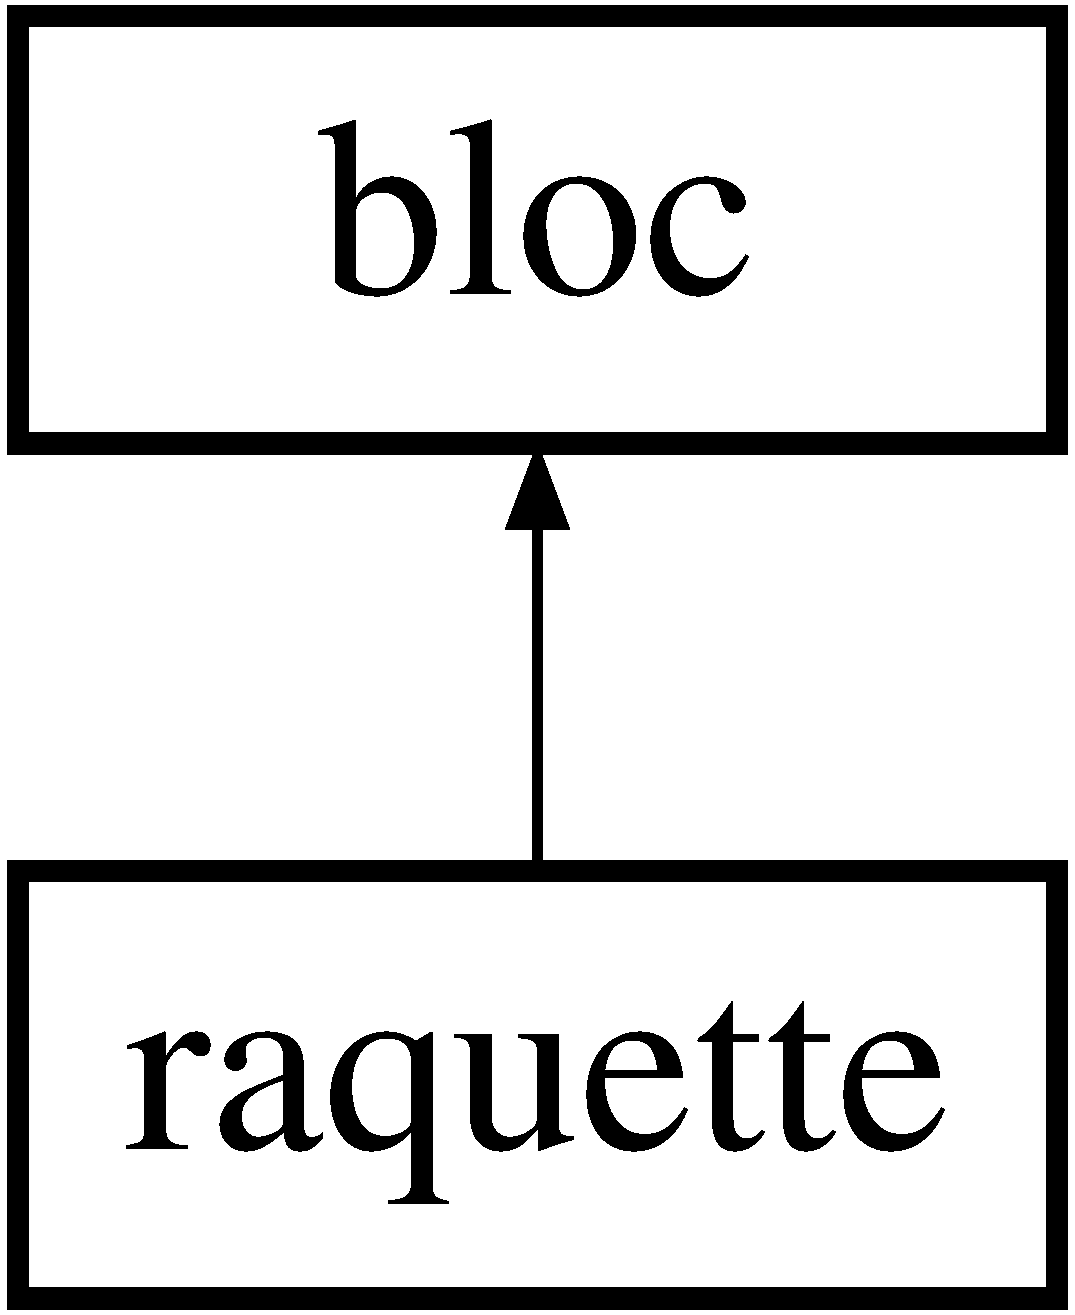
\includegraphics[height=2.000000cm]{classraquette}
\end{center}
\end{figure}
\subsection*{Public Member Functions}
\begin{DoxyCompactItemize}
\item 
\hypertarget{classraquette_ae8d1bbdc269988d69744c2279e6fdb21}{{\bfseries raquette} (float origine\-\_\-x, float origine\-\_\-y, float Longeur, float Hauteur, float r\-\_\-x, float r\-\_\-y)}\label{classraquette_ae8d1bbdc269988d69744c2279e6fdb21}

\item 
\hypertarget{classraquette_ad27917229e057c6131ef829eb5060e7a}{void {\bfseries change\-\_\-haut\-\_\-gauche} (\hyperlink{structvec2}{vec2} const \&nvl\-\_\-posi)}\label{classraquette_ad27917229e057c6131ef829eb5060e7a}

\end{DoxyCompactItemize}
\subsection*{Public Attributes}
\begin{DoxyCompactItemize}
\item 
\hypertarget{classraquette_aa9116c7e8a4f6f624a7489373c142b24}{float {\bfseries angle\-\_\-x}}\label{classraquette_aa9116c7e8a4f6f624a7489373c142b24}

\item 
\hypertarget{classraquette_a123b38337c44f8a99b9c32332c8ee484}{float {\bfseries angle\-\_\-y}}\label{classraquette_a123b38337c44f8a99b9c32332c8ee484}

\end{DoxyCompactItemize}


The documentation for this class was generated from the following files\-:\begin{DoxyCompactItemize}
\item 
raquette.\-hpp\item 
raquette.\-cpp\end{DoxyCompactItemize}

\hypertarget{classrender__area}{\section{render\-\_\-area Class Reference}
\label{classrender__area}\index{render\-\_\-area@{render\-\_\-area}}
}
Inheritance diagram for render\-\_\-area\-:\begin{figure}[H]
\begin{center}
\leavevmode
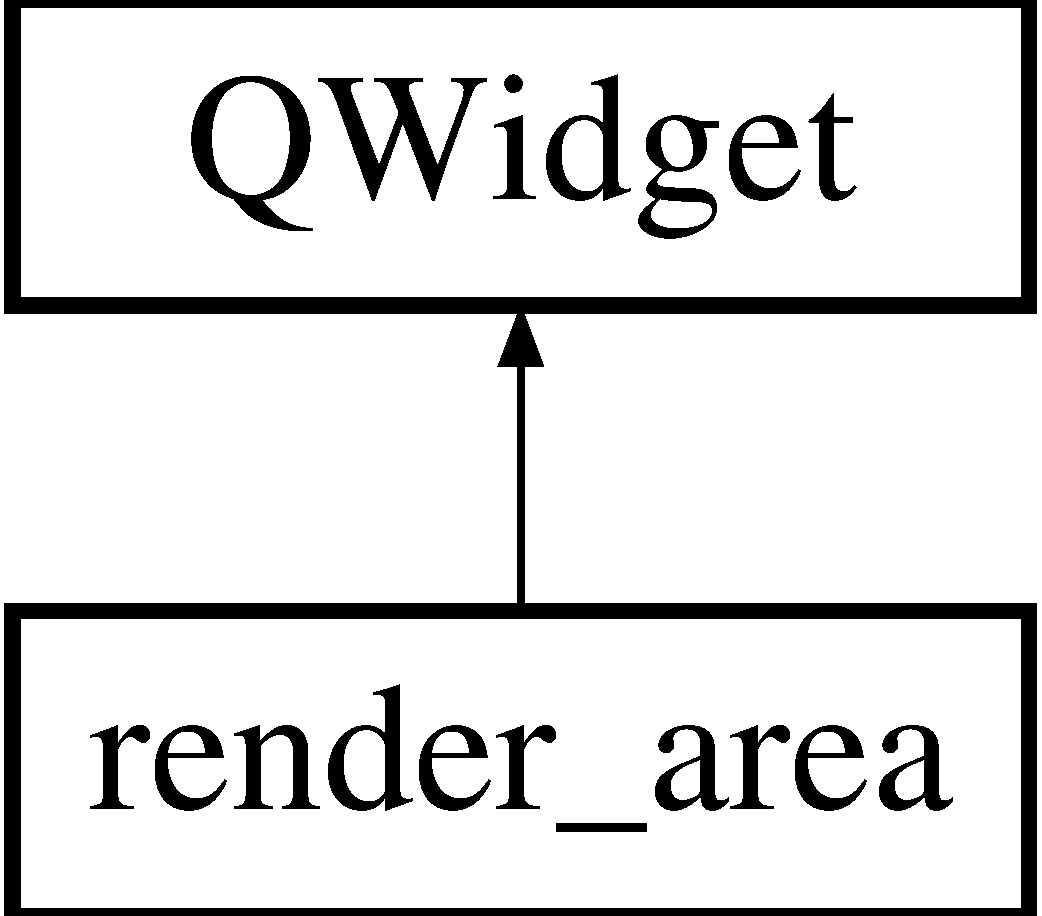
\includegraphics[height=2.000000cm]{classrender__area}
\end{center}
\end{figure}
\subsection*{Public Member Functions}
\begin{DoxyCompactItemize}
\item 
\hypertarget{classrender__area_a94fbfdd96b16ac545bcc551c1fd37b8c}{{\bfseries render\-\_\-area} (Q\-Widget $\ast$parent=0)}\label{classrender__area_a94fbfdd96b16ac545bcc551c1fd37b8c}

\item 
void \hyperlink{classrender__area_a3a5d00ec1ab31659f8b5d09fbd4ac910}{change\-\_\-draw\-\_\-circle\-\_\-state} ()
\item 
void \hyperlink{classrender__area_a02d5dad4e73fe27226ca173d6fe6cbaf}{set\-\_\-damping} (float damping)
\item 
void \hyperlink{classrender__area_abfb41f3e1ea6655e643c35decf895574}{set\-\_\-bounce\-\_\-coeff} (float bounce\-\_\-coeff\-\_\-value)
\item 
void \hyperlink{classrender__area_a1a04cb64fc5e810d4c4b6d537e493c9c}{setup\-\_\-bounce\-\_\-number} (Q\-Label $\ast$bounce\-\_\-number\-\_\-param)
\end{DoxyCompactItemize}
\subsection*{Protected Member Functions}
\begin{DoxyCompactItemize}
\item 
void \hyperlink{classrender__area_a3e0c5624174bac8f62fb07fff6258a0b}{paint\-Event} (Q\-Paint\-Event $\ast$event)
\item 
void \hyperlink{classrender__area_abf4d8df609e70aa6f523836ae00dde5d}{mouse\-Press\-Event} (Q\-Mouse\-Event $\ast$event)
\item 
void \hyperlink{classrender__area_a2552b2a7f1aa521bc8ded21e5bb6e2a7}{mouse\-Move\-Event} (Q\-Mouse\-Event $\ast$event)
\item 
void \hyperlink{classrender__area_a886281d1f08072563562c943493c0d5a}{mouse\-Release\-Event} (Q\-Mouse\-Event $\ast$event)
\end{DoxyCompactItemize}


\subsection{Member Function Documentation}
\hypertarget{classrender__area_a3a5d00ec1ab31659f8b5d09fbd4ac910}{\index{render\-\_\-area@{render\-\_\-area}!change\-\_\-draw\-\_\-circle\-\_\-state@{change\-\_\-draw\-\_\-circle\-\_\-state}}
\index{change\-\_\-draw\-\_\-circle\-\_\-state@{change\-\_\-draw\-\_\-circle\-\_\-state}!render_area@{render\-\_\-area}}
\subsubsection[{change\-\_\-draw\-\_\-circle\-\_\-state}]{\setlength{\rightskip}{0pt plus 5cm}void render\-\_\-area\-::change\-\_\-draw\-\_\-circle\-\_\-state (
\begin{DoxyParamCaption}
{}
\end{DoxyParamCaption}
)}}\label{classrender__area_a3a5d00ec1ab31659f8b5d09fbd4ac910}
Draw or not the circle when called \hypertarget{classrender__area_a2552b2a7f1aa521bc8ded21e5bb6e2a7}{\index{render\-\_\-area@{render\-\_\-area}!mouse\-Move\-Event@{mouse\-Move\-Event}}
\index{mouse\-Move\-Event@{mouse\-Move\-Event}!render_area@{render\-\_\-area}}
\subsubsection[{mouse\-Move\-Event}]{\setlength{\rightskip}{0pt plus 5cm}void render\-\_\-area\-::mouse\-Move\-Event (
\begin{DoxyParamCaption}
\item[{Q\-Mouse\-Event $\ast$}]{event}
\end{DoxyParamCaption}
)\hspace{0.3cm}{\ttfamily [protected]}}}\label{classrender__area_a2552b2a7f1aa521bc8ded21e5bb6e2a7}
Function called when the mouse is moved \hypertarget{classrender__area_abf4d8df609e70aa6f523836ae00dde5d}{\index{render\-\_\-area@{render\-\_\-area}!mouse\-Press\-Event@{mouse\-Press\-Event}}
\index{mouse\-Press\-Event@{mouse\-Press\-Event}!render_area@{render\-\_\-area}}
\subsubsection[{mouse\-Press\-Event}]{\setlength{\rightskip}{0pt plus 5cm}void render\-\_\-area\-::mouse\-Press\-Event (
\begin{DoxyParamCaption}
\item[{Q\-Mouse\-Event $\ast$}]{event}
\end{DoxyParamCaption}
)\hspace{0.3cm}{\ttfamily [protected]}}}\label{classrender__area_abf4d8df609e70aa6f523836ae00dde5d}
Function called when the mouse is pressed \hypertarget{classrender__area_a886281d1f08072563562c943493c0d5a}{\index{render\-\_\-area@{render\-\_\-area}!mouse\-Release\-Event@{mouse\-Release\-Event}}
\index{mouse\-Release\-Event@{mouse\-Release\-Event}!render_area@{render\-\_\-area}}
\subsubsection[{mouse\-Release\-Event}]{\setlength{\rightskip}{0pt plus 5cm}void render\-\_\-area\-::mouse\-Release\-Event (
\begin{DoxyParamCaption}
\item[{Q\-Mouse\-Event $\ast$}]{event}
\end{DoxyParamCaption}
)\hspace{0.3cm}{\ttfamily [protected]}}}\label{classrender__area_a886281d1f08072563562c943493c0d5a}
Function called when the button of the mouse is released \hypertarget{classrender__area_a3e0c5624174bac8f62fb07fff6258a0b}{\index{render\-\_\-area@{render\-\_\-area}!paint\-Event@{paint\-Event}}
\index{paint\-Event@{paint\-Event}!render_area@{render\-\_\-area}}
\subsubsection[{paint\-Event}]{\setlength{\rightskip}{0pt plus 5cm}void render\-\_\-area\-::paint\-Event (
\begin{DoxyParamCaption}
\item[{Q\-Paint\-Event $\ast$}]{event}
\end{DoxyParamCaption}
)\hspace{0.3cm}{\ttfamily [protected]}}}\label{classrender__area_a3e0c5624174bac8f62fb07fff6258a0b}
Actual drawing function \hypertarget{classrender__area_abfb41f3e1ea6655e643c35decf895574}{\index{render\-\_\-area@{render\-\_\-area}!set\-\_\-bounce\-\_\-coeff@{set\-\_\-bounce\-\_\-coeff}}
\index{set\-\_\-bounce\-\_\-coeff@{set\-\_\-bounce\-\_\-coeff}!render_area@{render\-\_\-area}}
\subsubsection[{set\-\_\-bounce\-\_\-coeff}]{\setlength{\rightskip}{0pt plus 5cm}void render\-\_\-area\-::set\-\_\-bounce\-\_\-coeff (
\begin{DoxyParamCaption}
\item[{float}]{bounce\-\_\-coeff\-\_\-value}
\end{DoxyParamCaption}
)}}\label{classrender__area_abfb41f3e1ea6655e643c35decf895574}
Set a new bouncing coefficient value \hypertarget{classrender__area_a02d5dad4e73fe27226ca173d6fe6cbaf}{\index{render\-\_\-area@{render\-\_\-area}!set\-\_\-damping@{set\-\_\-damping}}
\index{set\-\_\-damping@{set\-\_\-damping}!render_area@{render\-\_\-area}}
\subsubsection[{set\-\_\-damping}]{\setlength{\rightskip}{0pt plus 5cm}void render\-\_\-area\-::set\-\_\-damping (
\begin{DoxyParamCaption}
\item[{float}]{damping}
\end{DoxyParamCaption}
)}}\label{classrender__area_a02d5dad4e73fe27226ca173d6fe6cbaf}
Set a new damping value \hypertarget{classrender__area_a1a04cb64fc5e810d4c4b6d537e493c9c}{\index{render\-\_\-area@{render\-\_\-area}!setup\-\_\-bounce\-\_\-number@{setup\-\_\-bounce\-\_\-number}}
\index{setup\-\_\-bounce\-\_\-number@{setup\-\_\-bounce\-\_\-number}!render_area@{render\-\_\-area}}
\subsubsection[{setup\-\_\-bounce\-\_\-number}]{\setlength{\rightskip}{0pt plus 5cm}void render\-\_\-area\-::setup\-\_\-bounce\-\_\-number (
\begin{DoxyParamCaption}
\item[{Q\-Label $\ast$}]{bounce\-\_\-number\-\_\-param}
\end{DoxyParamCaption}
)}}\label{classrender__area_a1a04cb64fc5e810d4c4b6d537e493c9c}
Pass the pointer of the label for the bouncing number 

The documentation for this class was generated from the following files\-:\begin{DoxyCompactItemize}
\item 
render\-\_\-area.\-hpp\item 
render\-\_\-area.\-cpp\end{DoxyCompactItemize}

\hypertarget{structvec2}{\section{vec2 Struct Reference}
\label{structvec2}\index{vec2@{vec2}}
}


{\ttfamily \#include $<$vec2.\-hpp$>$}

\subsection*{Public Member Functions}
\begin{DoxyCompactItemize}
\item 
\hyperlink{structvec2_ae12a1a221eca3561809600a11b58eaa3}{vec2} ()
\item 
\hyperlink{structvec2_af5ad0dca7c4ac2f183f1df6792d1b94f}{vec2} (float x\-\_\-param, float y\-\_\-param)
\end{DoxyCompactItemize}
\subsection*{Public Attributes}
\begin{DoxyCompactItemize}
\item 
float \hyperlink{structvec2_a002d3519d48fe3cd79729b5b0ded74bf}{x}
\item 
float \hyperlink{structvec2_a6d28b12b511da692550fc9d37b4e9b1d}{y}
\end{DoxyCompactItemize}


\subsection{Detailed Description}
A 2\-D vector 

\subsection{Constructor \& Destructor Documentation}
\hypertarget{structvec2_ae12a1a221eca3561809600a11b58eaa3}{\index{vec2@{vec2}!vec2@{vec2}}
\index{vec2@{vec2}!vec2@{vec2}}
\subsubsection[{vec2}]{\setlength{\rightskip}{0pt plus 5cm}vec2\-::vec2 (
\begin{DoxyParamCaption}
{}
\end{DoxyParamCaption}
)}}\label{structvec2_ae12a1a221eca3561809600a11b58eaa3}
Constructor vec (0,0) \hypertarget{structvec2_af5ad0dca7c4ac2f183f1df6792d1b94f}{\index{vec2@{vec2}!vec2@{vec2}}
\index{vec2@{vec2}!vec2@{vec2}}
\subsubsection[{vec2}]{\setlength{\rightskip}{0pt plus 5cm}vec2\-::vec2 (
\begin{DoxyParamCaption}
\item[{float}]{x\-\_\-param, }
\item[{float}]{y\-\_\-param}
\end{DoxyParamCaption}
)}}\label{structvec2_af5ad0dca7c4ac2f183f1df6792d1b94f}
Constructor vec (x,y) 

\subsection{Member Data Documentation}
\hypertarget{structvec2_a002d3519d48fe3cd79729b5b0ded74bf}{\index{vec2@{vec2}!x@{x}}
\index{x@{x}!vec2@{vec2}}
\subsubsection[{x}]{\setlength{\rightskip}{0pt plus 5cm}float vec2\-::x}}\label{structvec2_a002d3519d48fe3cd79729b5b0ded74bf}
x coordinate \hypertarget{structvec2_a6d28b12b511da692550fc9d37b4e9b1d}{\index{vec2@{vec2}!y@{y}}
\index{y@{y}!vec2@{vec2}}
\subsubsection[{y}]{\setlength{\rightskip}{0pt plus 5cm}float vec2\-::y}}\label{structvec2_a6d28b12b511da692550fc9d37b4e9b1d}
y coordinate 

The documentation for this struct was generated from the following files\-:\begin{DoxyCompactItemize}
\item 
vec2.\-hpp\item 
vec2.\-cpp\end{DoxyCompactItemize}

\hypertarget{classwindow}{\section{window Class Reference}
\label{classwindow}\index{window@{window}}
}


{\ttfamily \#include $<$window.\-hpp$>$}

Inheritance diagram for window\-:\begin{figure}[H]
\begin{center}
\leavevmode
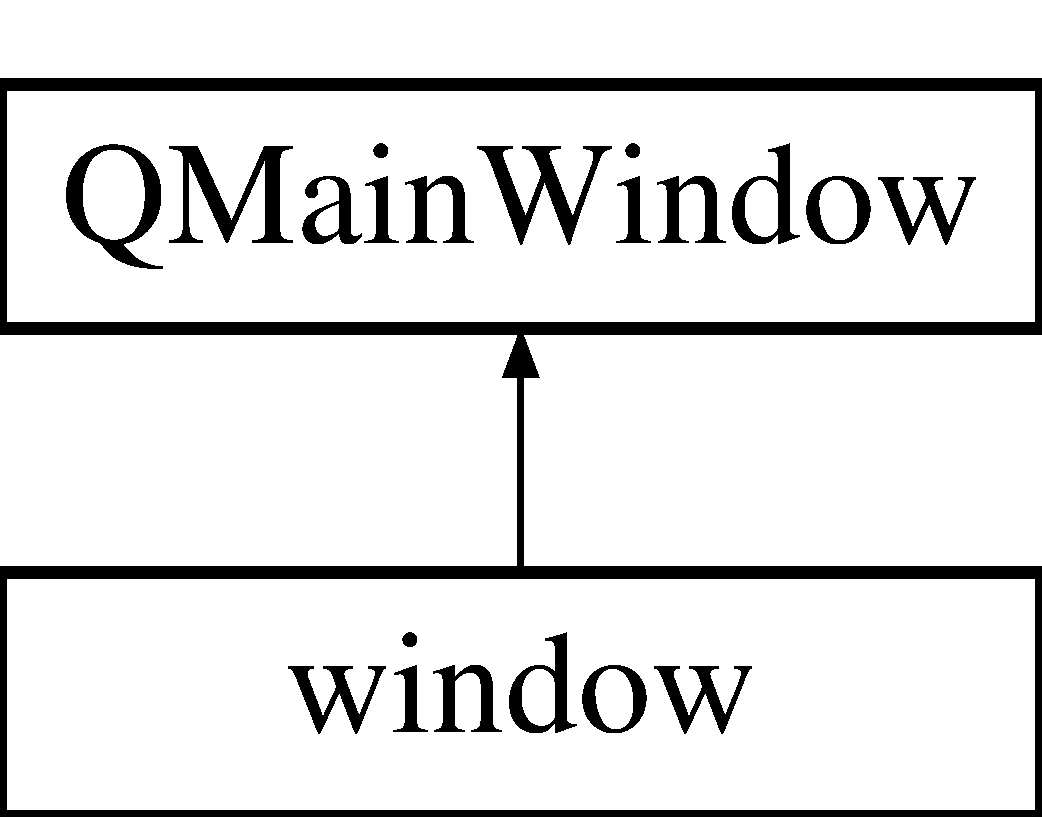
\includegraphics[height=2.000000cm]{classwindow}
\end{center}
\end{figure}
\subsection*{Public Member Functions}
\begin{DoxyCompactItemize}
\item 
\hypertarget{classwindow_ace6edf1b8b23a3ef56469995f289c87f}{{\bfseries window} (Q\-Widget $\ast$parent=nullptr)}\label{classwindow_ace6edf1b8b23a3ef56469995f289c87f}

\end{DoxyCompactItemize}


\subsection{Detailed Description}
Declaration of the window class 

The documentation for this class was generated from the following files\-:\begin{DoxyCompactItemize}
\item 
window.\-hpp\item 
window.\-cpp\end{DoxyCompactItemize}

%--- End generated contents ---

% Index
\newpage
\phantomsection
\addcontentsline{toc}{part}{Index}
\printindex

\end{document}
